\chapter{Introduction and background}
\label{ch-intro}

\section {A brief overview}
Predicting how neutral particle radiation moves through space and time is important when modeling inertial confinement fusion systems, pulsed neutron sources, and nuclear criticality safety experiments, among other systems.
Simulating these problems is computationally difficult using any numerical method, as the neutron distribution is a function of seven independent variables: three in space, three in velocity, and time.
% This problem demands HPCs and specifically the exascale
Modern HPC systems now enable high-fidelity simulation of neutron transport for problem types that have seldom been modeled before due to limitations of previous computers. % need citation?
Exploration of both novel numerical methods that can better take advantage of modern HPCs and the methods of implementing them in code are warranted.
% Specifically, large scale, highly dynamic transport problems require thousands of compute nodes using modern hardware accelerators (i.e., GPUs) \cite{hamilton_continuous-energy_2019, romano_openmc_nodate}.

My research is broad in its application but thematically specific, to satiate the ever-present need to go faster: faster and more accurate numerical methods, and faster implementations of numerical methods into HPC-worthy code.
I will first present my research questions, then provide more introduction to demonstrate the gaps in knowledge they seek to probe.
Then I will present my itemized research objectives and tasks required to implement those objectives.
I will briefly describe the methods already implemented and more thoroughly describe methods yet to be done.
Finally I will present preliminary results and draw initial conclusions.

This proposal is heavily supplemented by publications included as appendices.
Explanations of methods and results is intentionally terse as to respect my committees' already generous time commitment and service.
On that note I extend my most heart-felt gratitude to you and am keen and eager for the lively conversations sure to ensue about the work that I love.

\hfill

with mutual respect,

Joanna Piper Morgan

\subsection{Research questions}
\begin{enumerate}
    \item Can relying on abstraction through using software libraries enable non-expert users to produce efficient-performing software for heterogeneous computing systems?
    \item Will a space-parallel deterministic iterative solution algorithm outperform the standard angle-parallel iterative algorithm on heterogeneous architectures?
    \item For deterministic neutron transport, does accounting for transient effects alter convergence rates of the iterative solution algorithms?
    \item Can information coming from a streaming-only problem be used to inform cell boundary information and increase convergence rates of a one-cell inversion iteration algorithm?
    \item How can alternative Monte Carlo tracking schemes (namely Woodcock or delta tracking) be used be used to converge the quantities of interest faster?
\end{enumerate}

% Some already answered MC question
% phrase as hypthisys or hyp to q

\section{Neutron transport}

Transport equations are, at their most fundamental,equations of continuity.
Due to their ubiquity in nature, transport equations are used to describe an incredible number of physical systems including fluid dynamics, chemical reactions, electromagnetism, energy, and heat transfer.
My research contained herein focuses on neutron radiation transport specifically, but could easily be applied to other neutral particles, most relevantly photons \cite{radheattrans2003, chandrasekhar1960radiative}.
In fact many of the methods of solution described in this document started as approximations for radiative heat transfer or photon transport.
%justifying my ME degree
Assuming no neutrons are being produced by fission, the neutron transport equation (NTE) takes the form of an intergro-partial differential Boltzmann-type equation with seven independent variables \cite{duderstadt_hamilton}.
As with any other continuity equation it is written as a set of sources (on the right) and sinks (on the left):
\begin{multline}
    \label{eq:fullNTE}
    \frac{1}{v(E)}\frac{\partial \psi(\boldsymbol{r}, E, \boldsymbol{\hat{\Omega}},t)}{\partial t} + \boldsymbol{\hat{\Omega}} \cdot \nabla \psi(\boldsymbol{r}, E, \boldsymbol{\hat{\Omega}},t) + \Sigma(r, E, t) \psi(\boldsymbol{r}, E, \boldsymbol{\hat{\Omega}},t) = \\
    \int_{4\pi}\int_{0}^{\infty}\Sigma_s(\boldsymbol{r}, E'\rightarrow E, \boldsymbol{\hat{\Omega}'} \rightarrow \boldsymbol{\hat{\Omega}}, t)
    \psi(\boldsymbol{r}, E, \boldsymbol{\hat{\Omega}},t) dE' d\boldsymbol{\hat{\Omega}'} +
    s(\boldsymbol{r}, E, \boldsymbol{\hat{\Omega}},t) \;,
\end{multline}
where $\psi$ is the angular flux, $v$ is the velocity of the particles, $\Sigma$ is the macroscopic total material cross section, $\Sigma_s$ is the macroscopic scattering cross section, $\boldsymbol{r}$ is the location of the particle in three-dimensional space, $\boldsymbol{\hat{\Omega}}$ is the direction of travel in three-dimensional space, $s$ is the source of new particles being produced, $t$ is the time, and $E$ is the energy of the particles for $\boldsymbol{r} \in V$, $\boldsymbol{\hat{\Omega}} \in 4\pi$, $0<E<\infty$, and $0<t$ \cite{duderstadt_hamilton}. We also prescribe the initial condition
\begin{equation}
    \psi(\boldsymbol{r}, E, \boldsymbol{\hat{\Omega}},0) = \psi_{initial}(\boldsymbol{r}, E, \boldsymbol{\hat{\Omega}})
\end{equation}
and the boundary condition
\begin{equation}
    \psi(\boldsymbol{r}, E, \boldsymbol{\hat{\Omega}},t) = \psi_{bound}(\boldsymbol{r}, E, \boldsymbol{\hat{\Omega}},t) \text{ for } \boldsymbol{r} \in \partial V \text{ and } \boldsymbol{\hat{\Omega}} \cdot \boldsymbol{n} < 0 \;.
\end{equation}
A number of additional implicit assumptions are needed for the validity of this equation and my research including: particle-particle interactions are rare and can be neglected, neutrons are points in space with no volume, collision events occur instantaneously, and nuclear properties are known \cite{lewis_computational_1984}.
This equation is commonly solved using both deterministic and Monte Carlo solution methods as analytic solutions are sparse.

\section{Deterministic methods}

To recast the neutron radiation transport equation (eq \ref{eq:fullNTE}) into a form solvable on digital computers continuous functions of space, time, angle, and energy must be discretized.
Due to the nature of the NTE (intergro-PDEy-ness) an iterative scheme is also required.
In this section I describe the discretizations and their assumptions for the 1D, time-dependent, multi-group solver proposed within this work.
I will also describe the two fixed-point iterative schemes that I implement and discuss gaps in previous work of deterministic iterative solvers.
My work with deterministic schemes can be separated into two categories:
\begin{enumerate}
    \item How to use software engineering libraries to implement work more efficiently (RQ 1); and
    \item Considering novel methods to converge the solution faster on modern hardware
    \begin{enumerate}
        \item A space-parallel iterative scheme on modern HPC GPUs (RQ2);
        \item How transient behavior impacts convergence of a space-parallel iterative scheme (RQ3); and
        \item How to accelerate the space-parallel iterative scheme to converge faster (RQ4)
    \end{enumerate}
\end{enumerate}

\subsection{S$_N$ approximation in angle}

The S$_N$ or discrete ordinance approximation turns the introgro-PDE describing radiation transport into a coupled (simultaneous) set of linear PDEs in each angular direction.
It was first formulated by Chandrasekhar to describe radiative heat transfer in stellar media \cite{chandrasekhar1960radiative}.
The S$_N$ approximation was soon applied to neutron transport by Carlson \cite{precise1971carlson}, Lee \cite{discrete1961lee}, and Lathrop \cite{discrete1966lathnrop}.
The method of discrete ordinance was also adapted to general radiative heat transfer by Fiveland \cite{three1988fiveland} and Truelove \cite{discrete1987truelove}.
%While this work is only concerned with the S$_N$ approximations another approximation using the method of moments and orthogonal spherical harmonics as basis functions can also be used to approximate the angular integral which gives rise to the P$_N$ approximations \cite{radheattrans1990}.

At this point it becomes necessary to describe the other governing assumptions I use in this work including:
slab geometry (1D-rectilinear coordinates), isotropic scattering and sources, as well as the multi-group assumption in energy distribution.
The methods I propose in this work are not restricted by these assumptions---and future work may extend the methods described herein to be valid for anisotropic distributions in angle and/or solutions on unstructured meshes----but are made here for simplicity.
In-fact I make specific decisions in this work with the underlying discretization schemes to allow for eventual extension to these regimes.

When applied to equation \ref{eq:fullNTE} the resulting initialization point for my work is described by
\begin{multline}
    \label{eq:sn_nte}
    \frac{1}{v_g} \frac{\partial \psi_{m,g}(x,t)}{\partial t} + \mu_m \frac{\partial \psi_{m,g}(x,t)}{\partial x} + \Sigma_g(x) \psi_{m,g}(x,t)  \\
     = \frac{1}{2} \left( \sum\limits_{g' = 0}^G \Sigma_{s, g'\to g}(x) \sum\limits_{n=1}^N w_n \psi_{n, g'}(x,t) + Q_g(x,t) \right) \;, \\
    \qquad g=1 \ldots G \;, \qquad m=1 \ldots N \;, \qquad t > 0 \;, \qquad x \in [0,X] \;,
\end{multline}
where $\psi$ is the angular flux, $t$ is time, $x$ is location in 1D space, $g$ refers to the group, $v$ is velocity, $w_m$ is angular quadrature weight, $\mu_m$ is the angular quadrature ordinate ($\cos(\hat{\Omega}_\theta)$), $m$ is the quadrature index, and $Q$ is the isotropic material source.
In this work I will exclusively use Gauss-Legendre quadrature, but if extended to higher dimensions other quadratures sets would be required to evaluate the double integral over both angular directions (e.g. level-symmetric). 
The initial and boundary conditions are again prescribed angular flux distributions:
\begin{equation*}
    \psi_{m,g}(x,0) = \psi_{m,0}(x), \qquad m=1 \ldots N \;,
\end{equation*}
\begin{equation*}
    \psi_{m,g}(0,t) = \psi_{m,L}(t), \qquad \mu_m >0 \;,
\end{equation*}
\begin{equation*}
    \psi_{m,g}(X,t) = \psi_{m,R}(t), \qquad \mu_m <0 \;.
\end{equation*}
From here additional discretization can be used to turn the continuous functions of angular flux, source, material data, and differential operators into numerical approximations.

\subsection{Time-Space discretization schemes}

To enable this work in both space and time, discretization schemes are needed to treat the differential operators and continuous functions.
As the goal of the research is for development on heterogeneous architectures communication to work ratio may become an issue.
Numerical algorithms that require lots of communication back and forth between the host (CPU) and device (GPU) will limit the maximum allowable performance for most GPU accelerators.
To abate this issue higher (second) order discretization schemes can be used to add to the compute work required in every iteration, thus improving the communication to work ratio.

Various classes of spatial discretizations can be used in radiation transport.
Finite difference, finite element, and finite volume methods are all often employed with the most common scheme being Diamond-Differencing $\mathcal{O}(2)$.
Diamond-Difference is popular as it is the only second order space discretization that uses a single interior (cell-averaged) degree of freedom; however it only works on orthogonal grids.
%Intended future investigation of the scheme in this research are into non-uniform meshes.
While I will not include that analysis in this work, I do want to leave that opportunity open in order to better mesh with the modern state of the art of transport solvers which is on unstructured girds.
Therefore, I used a finite volume scheme specifically designed for use on unstructured grids called corner-balance, which was originally developed by Adams~\cite{adams_subcell_1997}.
It is a finite volume method and enforces conservation within subcell volumes in a spatial cell.
Simple corner balance was determined to be sufficient as it is higher $\mathcal{O}(2)$ order.
%Simple corner blance is not acrurate in the thin-limit however a slight alteration to it 
In 1-D slab geometry, simple corner balance is equivalent to the lumped-linear discontinuous finite element method.

Solving the transport equation with deterministic methods typically involves iterative schemes to converge the scattering source and transport operators (this is discussed more in section \ref{sec:intro_itterative-scheme}).
Thus implicit time marching schemes are often used to time step as they have desirable stability properties.
Specifically, implicit (backward) Euler $\mathcal{O}(1)$ or Crank-Nicolson $\mathcal{O}(2)$ are the most often employed.
%These schemes are advantageous as they often act like a wrapper around a steady state deterministic transport solver with few changes needed to implement.
While Crank-Nicolson is second order accurate it is not robust and can produce negative solutions and spurious osculations.
Time dependent multiple balance (TDMB) was derived by Variansyah, Larsen, and Martin~\cite{variansyah_robust_2021} to be a robust higher (second) order time discretization scheme.
TDMB is developed from the physics informed "multiple-balance" approach which has also been developed as a space discretization scheme.
When implementing a higher order method to allow for greater work-to-communicate ratios I decided to use this scheme. 

\subsection{Source-iteration}
\label{sec:intro_itterative-scheme}

The transport equation requires some kind of iterative scheme to converge the linkage between scattering source and transport operators.
The source iteration (SI) method is commonly used to do this, often accompanied by preconditioners or synthetic accelerators, where the contribution to the solution from the scattering source (summation in the RHS of equation \ref{eq:sn_nte}) is allowed to lag, while the angular flux is solved in every ordinate via transport sweeps through the spatial domain \cite{adams_subcell_1997}.
SI sweeps in Cartesian geometries are readily parallelized over the number of angles, as the source term is known from the previous iteration, allowing the angular flux in each ordinate to be computed independently. 
While any parallelization is a boon to performance, a scheme that is embarrassingly parallel over the dimension with the greatest number of degrees of freedom---space---may be advantageous.
In a single spatial dimension SI is \textit{annoying serial} in space and cannot be parallelized.

In higher spatial dimensions, many S$_N$ production codes that implement SI use some kind of wavefront marching parallel algorithm also known as a Kockh-Baker-Alcouff scheme \citep{KBA} also called "full parallel sweeps" in literature.
In this scheme a sweep begins in a spatial location where all cell dependencies are known from boundary information (e.g. a corner).
From there on a hypothetical 2D grid, the two nearest neighbor cells are computed independently, potentially in parallel; the next step would be 4 cells.
This diagonally expanding wavefront continues to march and is able to better parallelize as many cells spatially as possible eventually saturating the number of work threads if the problem is large enough.
%On CPUs this has been shown to be performant but this changing amount of work is not optimal on GPUs where.
%Performance evaluations of production codes that implement KBA on GPUs is sparse in literature and when avaliable is from proxy-apps.
%Ardra has such a proxy app 
%KBA algorithms are also tricky to efficiently implement in domain decomposed where wave front propagation between boundaries can be tricky.
%While this work is concerned with 1 spatial dimension when analyzing the state of the art it is important to consider that this is done.

%This has proven successful in modern transport applications on CPUs 
%(e.g., PARTISN, which implements the Koch--Baker--Alcouffe or KBA algorithm). 
%The state of the art in deterministic S$_N$ radiation transport is multi-group in energy distribution, diamond differencing first order space discretizations or other FEM FVM schemes on unstructured meshes, backward euler time stepping, domain decomposition via parallel block Jacobi, wave front marching schemes like KBA in higher spatial dimensions within a subdomain, and source iterations with diffusion synthetic acceleration (DSA) and potentially accompanied by GMRES solvers. Some examples of production codes that implement this are Partisn, Ardra, Minerate, Capsaicin, Denovo, Silver Fir, etc.
%Here again this is included as a
%Each one of these points becomes more difficult to implement due to angle-parallel SI with KBA, for example domain decomposition 

%Published literature on what schemes are implemented, how and their performance on GPU accelerators is sparse.
%Most of my understanding of what is currently used comes from conversations held at conferences with the developers of the codes themselves.
%One place I was able to find performance data on is a mini-app called Kripky \citep{kunen_kripke_2015}.
%Kripke is the publicly distributed version of Ardra that has performance data available.
%Roofline anylisys of Kripke has been published for performance on an AMD MI200 GPUs \citep{wolfe2022roofline}. 
%Specific k
%We conject that this is due to the nonlinear work load a wavefront marching schemes incurred. 


\subsection{One cell inversion-iteration}

% Intro to OCI and previous work including warsaw 

One Cell Inversions (OCI) (also called cell-wise parallel block Jacobi) is an alternative to SI where all angular fluxes in all ordinates and groups within a cell are computed in a single linear algebra step.
It assumes that the angular fluxes incident on the surfaces of the cell are known from a previous iteration.
OCI allows for parallelizing over the number of cells as each cell is solved independently of the others in a parallel.

Rosa Warsaw and Perks (2013) \cite{rosa_cellwise_2013} previously investigated OCI as a potentially superior iterative scheme over SI on vectroized heterogeneous architectures.
They supposed that because of the parallelism over the dominant domain, inherit data locality, ability to take advantage of LAPACK type libraries, and highly floppy operations present in an OCI type algorithm, it might out-perform an SI based implementation in wall clock runtime.
The study was conducted on state of the art (at the) time RoadRunner super computer at Los Alamos National Lab and took advantage of its 64 bit PowerXCell vectorized accelerator---a precursor to GPGPUs seen in HPCs today.
Rosa et al. implemented OCI in a 2D, multi-group, steady state, code using first order diamond differencing to discretize space, a multi-group scheme in energy distribution, and parallel block Jacobi and Gauss-Sidle iterations.

The authors concluded that the acceleration seen per-iteration in OCI was not enough to make up for the decay in convergence rate that OCI incurs.
As there is no communication of information between cells within an iteration (sometimes called a-synchronicity), OCI can require more iterations to converge to a solution for some of problems. 
Specifically, as cellular optical thickness goes down, OCI's relative performance degrades with a spectral radius not bounded by one independent of scattering ratio.
Figure~\ref{fig:specrad} illustrates this behavior, showing the spectral radii of the two iteration schemes as a function of cell thickness (in mean free path) and the scattering ratio.
These values were computed numerically from an infinite medium problem (via reflecting boundaries) using steady-state calculations in S$_4$. 
The smaller the spectral radius, the faster a method is converging.
The spectral radius for SI depends linearly on the scattering ratio, and for problems that are many mean free paths in size, it is nearly independent of cell optical thickness. 
The spectral radius of OCI decreases substantially as the optical thickness of the cells increases.
\begin{figure}[!htb]
    \centering
    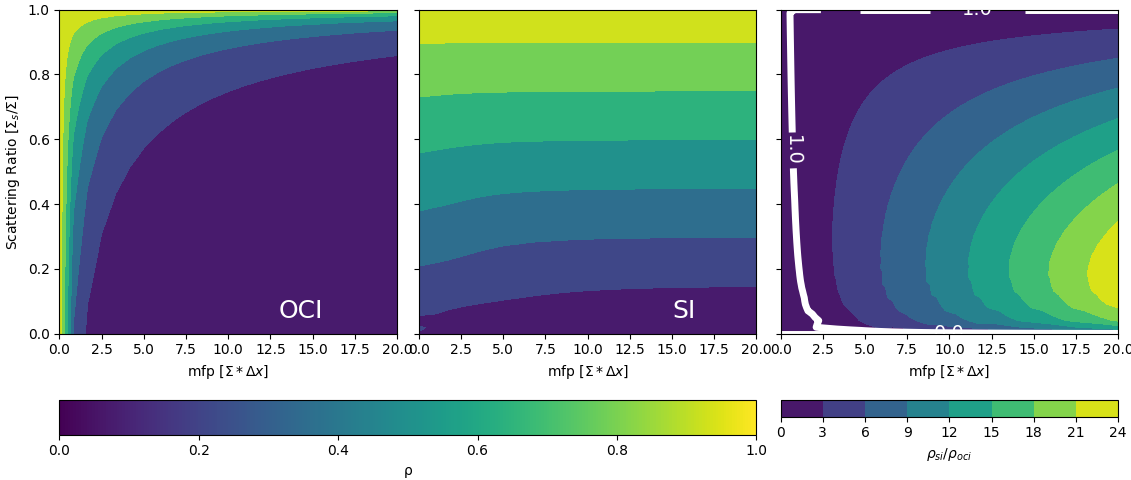
\includegraphics[width=(.9\textwidth)]{figures/spec_rad.png}
    \caption{Spectral radii ($\boldsymbol{\rho}$) of OCI (left) and SI (middle) and the ratio between the two (right), where $\boldsymbol{\Sigma}$ is the total cross section, $\boldsymbol{\Delta x}$ is the cell width, and $\boldsymbol{\Sigma_s}$ is the scattering cross section}
    \label{fig:specrad}
  \end{figure}
Rosa et al. also suggested that future developments in GPGPU accelerators might overcome this convergence rate decay for problems of interest.
The idea there as that even though more iterations will be required to converge a solution those iterations will be able to be done sufficiently faster (in wall-clock-runtime) to mean a solution is computed faster (again in wall clock runtime) then source iterations.

Other investigations have explored OCI as an acceleration scheme for SI \cite{anistratov_iterative_2015, hoagland_hybrid_2021}. %and a solution to the integral transport matrix method \citep{raffi2108pidotscom} and in the inexact parallel Jacobi scheme.
Previous investigations of OCI as an iterative scheme have been limited to steady state computations.

% potential transient effects in the thin limit 
%When solving discrete ordnance problems for transient systems many codes have implemented Crank-Nicholson or backward Euler time stepping.
%These schemes are non-intrusive often looking like an additional time marching loop around the already implemented transport infrastructure.
Regardless of the time stepping method an OCI iterative algorithm might come with some added befits when used in a transient scheme.
Returning to OCI's spectral radius shown at left in Fig.~\ref{fig:specrad}, since both dimensions are governed by relationships with the cross section of the cell ($\Sigma$), altering that value will impact convergence behavior. 
As the scattering ratio decreases, both iterative algorithms require fewer iterations to converge.
However, the spectral radius of OCI also decreases with increasing optical thickness, \textit{which is an added benefit}.
When solving optically thick and highly scattering problems, small increases in $\Sigma$ may drastically improve the relative performance of OCI in comparison with SI.
%Physically this can be understood as single particles living in single cells for many more iterations.
Time step and cellular optical thickness are inversely proportional to each other, meaning a smaller time step will yield a larger effective total cross section, thus theoretically improving the spectral radius.
This behavior is not expected to happen in source iterations as SI does not directly depend on cellular optical thickness---behaving linearly in that dimension for all but the most thick problems.

\subsection{Synthetic acceleration}
% acceleration schemes for SI
In order to converge iterative schemes faster many synthetic acceleration techniques have been explored and implemented over the years \cite{adams_fast_2002}.
The most common used in conjunction with source iterations is diffusion synthetic acceleration (DSA) which converges the slowest mode of SI---the so called diffusive-limit \cite{adams_fast_2002}.
The failure of SI in the diffusive limit can be physically understood as there is no linking between angles within an iteration and a diffusive problem is a coupling of angles.
DSA adds a mid-step correction term based off of a cheap to compute diffusion approximation of transport effects.
Other synthetic acceleration techniques include quasi-diffusion and Boundary projection acceleration \cite{adams_fast_2002}.

% acceleration schemes for OCI
Much less work has gone into exploring synthetic acceleration techniques for one cell inversions.
The slowest mode of convergence of OCI is known to be the thin limit due to the a-synchronicity of the scheme (lagging cell-wise boundary fluxes) \cite{hoagland_hybrid_2021}.
The spectral radius will decay unbounded in the thin limit, regardless of scattering ratio \cite{rosa_cellwise_2013}.
Rosa and Warsa (2009) investigated using transport synthetic acceleration (TSA) as the low order synthetic accelerator via fourier analysis \cite{tsa2009rosa, tsa_slab2006rosa, tsa_2d2007rosa}.
TSA uses a low order transport sweep with potentially fewer angles (when accompanied by SI) and a smaller scattering ratio (often controlled by the user by term $\beta \in [0,1]$) to inform the error correction equation \cite{tsa1997gilles}.
In effect TSA is just a less expensive transport sweep, but a transport sweep none-the-less and comes with all the baggage I am trying to avoid of a transport sweep.
Rosa and Warsa say as much when they suggest a scheme where TSA is only "turned on" after a given number of iterations fails to converge to a solution \cite{tsa2009rosa}.
%TSA
%While they suggest future work to implement, no published results of an OCI+TSA scheme.

% gmres
Both SI and OCI are forms of a fixed-point (or Richardson) iteration that use different operator splittings.
In a fixed-point iteration an initial guess of the angular or scalar flux is supplied as a known to the solver which in turn returns an angular or scalar flux.
This becomes the new guess and is iterated until the relative error between the guess and the output falls to below a given tolerance \cite{lewis1984computational}.
Kyrlov methods on the other hand store multiple copies of the ``guess" as to compute the next guess in a way that is orthogonal of the previous \cite{gmres1996kelley, patton_application_2002}.
Generalized minimal residual method (GMRES) specifically, has been shown to make DSA schemes that preform relatively poorly, work well \cite{kylov2004warsa}.
%They work by keeping copies of the guess for a given number of previous iterates, compute residuals and ensure the next guess is orthogonal to the previous ones\cite{subspace2004warsa}.

\subsection{Novelty and relation to research questions}

The hypothesized additional benefit of of OCI in a time dependent code (RQ 3) coupled with the vast improvements in GPGPU accelerators in the past decade since Rosa et al. \cite{rosa_cellwise_2013} conducted their investigations (RQ 1 and 2), along with the ability to explore higher order spatial and transient discretization schemes (RQ 2) motivates the first publication associated with this work.
After that an exploration of a synthetic acceleration algorithm to converge OCI in the thin limit will become the second (RQ 4).
%Furthermore, as previously mentioned, source iterations are often implemented in production accompanied by some kind of synthetic-acceleration scheme or other preconditioner to converge it's slowest converging mode (the diffusive limit).
%OCI has never been implemented with a prevonditon

\section {Monte Carlo methods}

%Predicting how neutrons move through space and time is important when modeling inertial confinement fusion systems, pulsed neutron sources, and nuclear criticality safety experiments, among other systems.

While deterministic schemes produce an exact solution to an inexact problem Monte Carlo methods provide an inexact solution---with an associated error---to an exact problem.
Monte Carlo methods can treat the independent variables of the NTE (space, angle, time, energy) as continuous, thus eliminating the discretization errors seen with deterministic methods.
The behavior of neutrons can be modeled with a Monte Carlo simulation, where pseudo-particles with statistical importance are created and transported to produce a particle history \cite{lewis_computational_1984}.
A particle's path and the specific set of events that occur within its history are governed by pseudo-random numbers, known probabilities (e.g., from material data), and known geometries.
Data about how particles move and/or interact with the system are tallied to solve for parameters of interest with an associated statistical error from the Monte Carlo process. 
The analog Monte Carlo method is slow to converge (with a convergence rate of $\mathcal{O}(1/\sqrt{n})$ where $n$ is the number of simulated particles).
New Monte Carlo schemes could converge the solution faster in wall-clock time with fewer simulated particles and may be needed to effectively simulate some systems.

%history with interesting citations
%Monte Carlo methods where orignal propased by Stanislaw Ulam in 1946 after work on the Manhattan project.
%It's orginal use in fact was the tracking neutrons thru phase space using handheld computers called Fermiacs.
%The challenge problem I seek to investate also dates back this time.
%Since then from a report in 1995 over 60\% of computational time on US Government super computing systems was concerend with converging the Monte Carlo method

% deception of the section
My work with Monte Carlo schemes---as with my deterministic work---is broadly divided into two categories
\begin{enumerate}
    \item How to use software engineering libraries to implement work more efficiently (RQ 1); and
    \item Considering novel methods to converge the solution faster on modern hardware (RQ 5).
\end{enumerate}
The first section digs into the first goal examining performance portability schemes in high level languages and the work that is currently deployed in Monte Carlo/Dynamic Code (MC/DC) as part of my work with the Center for Exascale Monte Carlo Neutron Transport (CEMeNT).
The second contains work initially done in a production code at Los Alamos National Laboratory and a proposed extension of the scheme the scheme in an implementation in MC/DC.

\subsection{Portability frameworks for Monte Carlo methods}

In this section I introduce initial investigations into high-level performance portability frameworks and discuss 
Developing software to simulate physical problems that demand high-performance computing (HPC) is difficult.
Modern HPCs commonly use both CPUs and GPUs from various vendors.
Years can be spent porting a code from CPUs to run on GPUs, then again when moving from one GPU vendor to the next \cite{pozulp_progress_2023}.
Portability issues compound when designing software for rapidly developing numerical methods where algorithms need to be both implemented and tested at scale.
Finding a software engineering approach that balances the need for portability, rapid development, open collaboration, and performance can be challenging especially when numerical schemes do not rely on commonly library implemented operations (i.e., linear algebra as in LAPACK or Intel MKL). 
% one paragraph for CISE reqirments

Common HPC software engineering requirements are often met using a Python-as-glue-based approach, where peripheral functionality (e.g., MPI calls, I/O) is implemented using Python packages but compiled functions are called through Python's C-interface where performance is needed.
Python-as-glue does not necessarily assist in the production of the compiled compute kernels themselves---what the Python is gluing together---but can go a long way in simplifying the overhead of peripheral requirements of HPC software.
With this technique, environment management and packaging uses \texttt{pip}, \texttt{conda}, or \texttt{spack}, input/output with \texttt{h5py}, MPI calls with \texttt{mpi4py}, 
and automated testing with \texttt{pytest}, which can all ease initial development and continued support for these imperative operations. 

Many tools have been developed to extend the Python-as-glue scheme to allow producing single-source compute kernels for both CPUs and GPUs.
% a DSL, pyfr
One tactic is to use a domain-specific language to avoid needing a low-level language (e.g., FORTRAN, C).
A domain-specific language is designed to alleviate development difficulties for a group of subject-area experts and can abstract hardware targets if defined with that goal.
%It can even abstract hardware targets if it is defined with that goal.
PyFR, for example, is an open-source computational fluid dynamics solver that implements a domain-specific language plus Python structure to run on CPUs and Nvidia, Intel, and AMD GPUs~\cite{pyfrPetascale}. 
%The overhead of this Python glue is less than 1\% in PyFR.
Witherden et al.~\cite{pyfrPetascale} discussed how this scheme allows PyFR developers to rapidly deploy numerical methods at deployment HPC scales and have demonstrated performance at the petascale.

Other projects have addressed the need to write user-defined compute kernels entirely in Python script.
Numba is a compiler that lowers a small subset of Python code with NumPy arrays and functions into LLVM, then just in time (JIT) compiles to a specific hardware target \cite{lam_numba_2015}. 
Numba also compiles global and device functions for Nvidia GPUs from compute kernels defined in Python.
API calls are made through Numba on both the Python side (e.g., allocate and move data to and from the GPU) and within compiled device functions (e.g., to execute atomic operations).
When compiling to GPUs, Numba supports an even smaller subset of Python, losing most of the operability with NumPy functions.
If functions are defined using only that smallest subset, Numba can compile the same functions to CPUs or GPUs, or execute those functions purely in Python.
Numba data allocations on the GPU can be consumed and ingested by functions from CuPy if linear-algebra operations are required in conjunction with user-defined compute kernels.

When targeting use of a Python portability scheme to HPC for neutron transport I compared the same algorithm in various implementations using PyKokkos \cite{AlAwarETAL21PyKokkos}, PyCUDA/PyOpenCL \cite{kloeckner_pycuda_2012}, and Numba \cite{morgan2022}.

%Numba has been shown to be slower then other high level portability frameworks for unoptimized matrix multiplication \cite{Godoy_2023}.
%Monte Carlo neutronic workflows are so memory bound that it's doubtful even significant changes to FLOP performance of a 


%
%I found that all three methods produced similar runtimes for our workflows on CPUs and GPUs for a simple transient Monte Carlo neutron transport simulation \cite{morgan2022}.
%Ultimately, we decided to use a Numba + mpi4py development scheme to build out a Monte Carlo neutron transport code for rapid numerical methods development, portable to various HPC architectures \cite{variansyah_mc23_mcdc,morgan_monte_2024,transport_cement_mcdc_2024} (RQ 1).

\subsection{Delta tracking}

Woodcock, or delta, tracking \cite{woodcock1965} is a variance-reduction technique that computes the majorant cross-section for the whole problem space, then uses this to determine a distance to collision for all particles.
Coupled with rejection sampling to sort for phantom collisions, and a collision estimator to compute scalar flux, delta tracking often improves performance over analogue Monte Carlo in problems that warrant it (problems with a long mean free path).
Many production Monte Carlo Neutron transport codes like Serpent \cite{Serpent2013, leppanen_use_2017, leppanen_performance_2010} and others \cite{delta2017rowland} use this method.
In traditional delta tracking first the macroscopic majorant cross section is computed for the entire problem space
\begin{equation}
    \label{eq:majorant}
    \Sigma_{M}(E) = \max\left(\Sigma_{T,b}(E), ..., \Sigma_{T,B}(E)\right) \,\text{,}
\end{equation}
where $E$ is energy, $\Sigma_{M}$ is the microscopic majorant cross-section, and $\Sigma_{T,b}$ is the microscopic total cross-section of the $=b^{\text{th}}$ material.
Now to sample a the distance to a collision
\begin{equation}
    \label{eq:sample}
    D = \frac{-\ln{\xi}}{\Sigma_{M}(E)} \, \text{,} 
\end{equation}
where $\xi\in[0,1]$.
If the potential collision occurs within the cell, we move the particle to the sampled distance and do rejection sampling, since we are now potentially forcing collisions that did not occur.
We sort out these phantom collisions by allowing particles to continue to a new sampled distance if
\begin{equation}
    \label{eq:reject}
    \xi < \frac{ \Sigma_{T,j}(E) } { \Sigma_M(E) } \, \text{,}
\end{equation}
where $\xi\in[0,1]$ is a new random number and $\Sigma_{T,j}(E)$ is the macroscopic total cross-section of the cell $j^{th}$ current cell.
Standard delta tracking is required to use a collision estimator which is less efficient then the normal track length estimator used in surface tracking\cite{mc2018}.
If I can find a way to use the track-length estimator while doing delta tracking we could improve the performance of a Monte Carlo code (RQ 5).

\if
\section{GPU and GPU performance Anylisi}
% Kripkey performance published in gray literature
When analyzing performance on GPUs the roofline performance model is often used.
The roof is constructed by the communication or bandwidth (Bytes/S) and computation resources of a specific GPU for a specific numerical precision (floating operation points per second or FLOPS).
As algorithms at their most optimized become performance limited by either bandwidth or compute resources.
Thus when the performance of a given GPU device function is on the roofline it is the most optimized it could be.

Performance anylisys on GPUs of deterministic sweep codes is limited in the literature. 
That is espically the case when looking for roofline anylisys specifically.
Roofline models have previously been used to evalueate some miniapps in the Monte Carlo world \citep{tramm2021domain, tramm2022roofline}.


As the wave moves through the problem space in a given ordinant the number of cells to be solved in parallel can change dramatically.
This kind of in kernel dynamic problem 
While our work is limited to a single spatial dimension thus avoiding anylisys of KBA algorithms this shows the state of the art in performance of deterministic code.
\fi